

\section{General automata and rational expressions}
\label{sec:aut-fct}

Automata are `labelled graphs', and these labels are, in full 
generality, elements of a monoid associated with a multiplicity 
(taken in a semiring), or a finite sum of such weighted elements.
% , or in some cases, a series over a monoid with 
% coefficients in a semiring.
The commands considered in this section make assumption neither on 
the monoid, nor on the weight semiring.
They are thus called by any instance of \tafkit, for automata of 
\emph{any type}.\footnote{%
   Allowing some exceptions, mentioned when describing the functions.} 



\renewcommand{\theenumii}{\theenumi.\arabic{enumii}}

\begin{enumerate}
    
\item Graph functions   

\begin{enumerate}
%     \addtocounter{enumii}{-1}
% \item \Fctaut{reverse}
\item \Fctaut{accessible}\vrglst \Fctaut{coaccessible}%, \Fctaut{is-accessible} 
%\item , \Fctaut{is-coaccessible}
\item \Fctaut{trim}, \Fctaut{is-trim}
\item \Fctaut{is-empty}
\item \Fctaut{is-useless}
\end{enumerate}
    
\item Transformations of automata

\begin{enumerate}
\item \Fctaut{proper}\vrglst \Fctaut{is-proper}
\item \Fctaut{standardize}\vrglst \Fctaut{is-standard}
% \item \Fctaut{normalize}, \Fctaut{is-normalized}
% \item \Fctaut{support}
% \item \Fctaut{characteristic}
\end{enumerate}

\item Operations on automata

\begin{enumerate}
\item \FctautD{union}
\item \FctautD{sum}
\item \FctautD{concatenate}
\item \Fctaut{star}
\item \Fctkaut{left-mult}\vrglst \Fctkaut{right-mult}
% \item \Fctkaut{right-mult}
\item \FctParD{chain}{aut}{n}
\end{enumerate}

\item Operations on behaviours of automata

\begin{enumerate}
\item \FctautD{sum-S}
\item \FctautD{cauchy-S}
\item \Fctaut{star-S}
\end{enumerate}

% \item Transformations of expressions
% 
% \begin{enumerate}
% \item \Fctexp{is-valid}, \Fctexp{cst-term}
% \item \Fctexp{has-finite-support}
% \end{enumerate}

\item Automata and expressions; operations on expressions

\begin{enumerate}
\item \Fctaut{aut-to-exp}\vrglst \Fctaut{aut-to-exp-DM}\vrglst 
\Fctaut{aut-to-exp-SO}
    \item \Fctexp{expand}
    % \item \FctexpD{sum-E}
    % \item \FctexpD{product-E}
    % \item \Fctexp{star-E}
    % \item \Fctkexp{left-mult-E}
    % \item \Fctkexp{right-mult-E}
\item \Fctexp{exp-to-aut}
\end{enumerate}
\end{enumerate}

\shortclear

\longonly{%
\begin{ComVd}{110724}
    
    \thi not implemented:
        
    the \code{is-} commands: \Fctaut{is-accessible}, 
    \Fctaut{is-coaccessible}.
    
    \thii transfered to other sections:
    
    \Fctaut{support}, \Fctaut{characteristic};

    \Fctexp{expand}.
	
	\thiii Implemented with a restricted scope: \Fctexp{exp-to-aut}.
    
    \thiv Hidden, not documented, but stil exist:

    \Fct{normalize}, \Fct{is-normalized}.

\end{ComVd}
}%

The following function is not implemented. It is 
just convenient to \emph{describe specification} of `dual' functions 
in this section. 
It differs from \Fct{transpose} as it has no effect on the labels.

\begin{SwClCmd}
\begin{shell}
$ \kbd{vcsn reverse a.xml > b.xml}
$
\end{shell}%
\end{SwClCmd}%
\begin{SwClTxt}
    Reverses every edge of the underlying graph of the automaton 
    \Prm{a.xml}, as well as exchanges the initial and final edges and 
    write the result in \Prm{b.xml}. 
\end{SwClTxt}%



\subsection{Graph functions}
\label{sec:gra-fct}

Automata are `labelled graphs': a number of functions on automata are  
indeed functions on the graph structure, irrespective of the labels.

\subsubsection{\Fct{accessible}, \Fct{coaccessible}}

\begin{SwClCmd}
\begin{shell}
$ \kbd{vcsn\footnotemark accessible a.xml > b.xml}
$
\end{shell}%
\end{SwClCmd}%
\begin{SwClTxt}
    Computes the accessible part of the automaton 
    \Prm{a.xml} and writes the result in \Prm{b.xml}.
\end{SwClTxt}%
\IndexFct{accessible}%
\index{automaton!accessible part of an --}%
\footnotetext{As the functions of this section are valid for all 
instances of \tafkitv, the instance in the description is shown under 
the generic name \code{vcsn}.}

\Spec
The description of the function is the specification.
It is realised by a traversal of the underlying graph of \Prm{a.xml}. 
It may imply a renumbering of the states.

\longonly{%
\Comt
In principle, this is a function about which it can be discussed 
whether it should be \emph{in place} or not. 
The choice may exist in the \vcsn library, but not in \tafkit where 
\emph{no function} is in place.
\index{place@in place function}%
}%

\medskip 
\begin{SwClCmd}
\begin{shell}
$ \kbd{vcsn coaccessible a.xml > b.xml}.
$
\end{shell}%
\end{SwClCmd}%
\begin{SwClTxt}
    Computes the co-accessible part of the automaton 
    \Prm{a.xml} and writes the result in \Prm{b.xml}.
\end{SwClTxt}%
\IndexFct{coaccessible}

\Spec
\Fctq{coaccessible}{a.xml} = \Fctq{reverse}{\Fctq{accessible}{\Fctq{reverse}{a.xml}}}


\subsubsection{\Fct{trim}, \Fct{is-trim}}

\begin{SwClCmd}
\begin{shell}
$ \kbd{vcsn trim a.xml > b.xml}
$
\end{shell}%
\end{SwClCmd}%
\begin{SwClTxt}
    Computes the trim part of the automaton 
    \Prm{a.xml} and writes the result in \Prm{b.xml}.
\end{SwClTxt}%
\IndexFct{trim}

\Spec
\Fctq{trim}{a.xml} = \Fctq{coaccessible}{\Fctq{accessible}{a.xml}}

\medskip 
\begin{SwClCmd}
\begin{shell}
$ \kbd{vcsn  -v is-trim a.xml}
Input is not trim
\end{shell}%
\end{SwClCmd}%
\begin{SwClTxt}
    Tells whether or not the automaton 
    \Prm{a.xml} is trim.
\end{SwClTxt}%
\IndexFctIs{trim}

\Spec
\Fctq{is-trim}{a.xml} = \Fctq{is-accessible}{a.xml} $\wedge$ 
\Fctq{is-coaccessible}{a.xml}\footnote{%
   Even if the functions \Fct{is-accessible} and 
   \Fct{is-coaccessible} are not implemented, the specification is 
   clear.}


\subsubsection{\Fct{is-empty}}

\begin{SwClCmd}
\begin{shell}
$ \kbd{vcsn -v is-empty a.xml}
Input is not empty
\end{shell}%
\end{SwClCmd}%
\begin{SwClTxt}
    Tells whether or not the automaton 
    \Prm{a.xml} is empty.
\end{SwClTxt}%
\IndexFct{is-empty}

\subsubsection{\Fct{is-useless}}

\begin{SwClCmd}
\begin{shell}
$ \kbd{vcsn -v is-useless a.xml}
Input is has successful computations
\end{shell}%
\end{SwClCmd}%
\begin{SwClTxt}
    Tells whether or not the automaton 
    \Prm{a.xml} has successful computations.
\end{SwClTxt}%
\IndexFct{is-useless}

\Spec
\Fctq{is-useless}{a.xml} = \Fctq{is-empty}{\Fctq{trim}{a.xml}}


\Comt
\Fct{is-useless} is a \emph{graph function} and tests whether there 
are \emph{successful computations} in the automaton, that is a 
sequence of co-terminal transitions, the first one beginning in an 
`initial state', the last one ending in a `final state'.
By definition, or by the way automata are specified in \vcsn, 
each of these transitions have a non-zero label.
This does not imply that the label of the computation itself is 
different from zero, nor that the behaviour of the automaton is 
different from zero.

For instance, the behaviour of the $\Z$-automaton \code{usl.xml} of 
\figur{usl} is the null series. 
Nevertheles one has:
\begin{shell}
$ \kbd{vcsn-char-z -v is-useless usl.xml}
Input has a successful computation
\end{shell}%$


\begin{figure}[ht]
    \centering
\includegraphics[scale=0.5]{figures/usl.ps}
\caption{The $\Z$-automaton \code{usl.xml}}
\label{fig:usl}
\end{figure}


\subsection{Transformations of automata}
\label{sec:tra-aut}

\subsubsection{\Fct{is-proper}, \Fct{proper}}
\label{ssc:aut-pro}%

\begin{SwClCmd}
\begin{shell}
$ \kbd{vcsn -v is-proper a.xml}
Input is not proper
\end{shell}%
\end{SwClCmd}%
\begin{SwClTxt}
    Tells whether or not the automaton 
       \Prm{a.xml} is proper.
\end{SwClTxt}%
\IndexFctIs{proper}%


\shortclear 
\Spec
An automaton is \emph{proper} if it has no \emph{spontaneous 
transitions},\footnote{%
   Often called also \emph{$\epsilon$-transitions}.}
that is, no transition labelled by the 
identity of the monoid (empty word for free monoids, the pair of 
empty words for product of free monoids).
If a transition is labelled by a polynomial and 
not by a monomial, this means that the support of the polynomial does 
not contain the identity.
\index{automaton!proper --}%
\index{spontaneous|see{transition}}%
\index{epsilon|see{transition}}%
\index{transition!spontaneous --}%
\index{transition!epsilon --}%

\medskip
\begin{SwClCmd}
\begin{shell}
$ \kbd{vcsn proper a.xml > b.xml}
$
\end{shell}%
\end{SwClCmd}%
\begin{SwClTxt}
    Computes a proper automaton equivalent to
    \Prm{a.xml} and writes the result in \Prm{b.xml}.
\end{SwClTxt}%
\IndexFct{proper}%

\Spec 
\thi This procedure can be called for automata of any type. 

\thii The procedure eliminates the \emph{spontaneous transitions} 
of the automaton. 
The result may not be defined for some automata of certain type.
For the consistency of the definitions in full generality we had to 
depart from the definition taken in~\cite{Saka03,Saka09} and consider 
a very restricted definition of \emph{validity} of an automaton 
(\cite{LombSaka12,LombSakaXX}.
For the weight semirings that are implemented in \tafkitv however,
the new definition of validity amounts to the old one and an 
automaton is valid if, and only if, the family of weights of 
computations labelled by the identity is \emph{summable}.

\thiii
The spontaneous-transition elimination algorithm implemented in 
\vcsnv is novel.
It is valid for automata whose weight semiring is \emph{positive} 
(such as~$\K=\B$, $(\Z,\min,+)$, $(\Z,\max,+)$) or \emph{ordered}, 
with a `positive' part which is a subsemiring and a `negative' part 
which is the opposite of tbe positive part
(such as~$\K=\Z$, $\Q$, $\R$).
Finally, the case of~$\K=\F_{2}$ is treated separately.

Altogether, the algorithm is valid for all instances of \tafkitv.
It is documented in~\cite{LombSaka12,LombSakaXX}.


\Exam
We test the algorithme \code{proper} with the automaton
\code{prp-tst1.xml} described below and represented at 
\figur{prp-tst}.
We run indeed the test with a varying weight~$k$ for the spontaneous 
transition~$3$ from state~$1$ to state~$2$ ($k=\frac{1}{2}$ in the 
illustration below).
\begin{shell}
$ \kbd{vcsn-char-q -aa edit prp-tst1.xml}
...
Automaton description:
  States: 0, 1, 2, 3
  Initial states: 0 (W: 1)
  Final states: 2 (W: 1)

  Transitions: 
    1: From 0 to 0 labeled by (\{1/2\} 1)
    2: From 0 to 1 labeled by a
    3: From 1 to 2 labeled by (\{1/2\} 1)
    4: From 2 to 1 labeled by 1
    5: From 2 to 3 labeled by 1
    6: From 3 to 1 labeled by (\{-1\} 1)
\end{shell}%
Although there exists always an order to eliminating the spontaneous 
transitions such that one gets a valid automaton, the behaviour of 
\code{prp-tst1.xml} itself is defined if, \emph{and only if}, $\msp k < \frac{1}{2} \msp$ 
 and this is to be detected by the algorithm.

\begin{figure}[ht]
    \centering
\includegraphics[scale=0.5]{figures/prp-tst.ps}
\caption{A test for the algorithm \code{proper}}
\label{fig:prp-tst}
\end{figure}


\subsubsection{\Fct{is-standard}, \Fct{standardize}}
\label{ssc:aut-sta}%

\begin{SwClCmd}
\begin{shell}
$ \kbd{vcsn -v is-standard a.xml}
Input is standard
\end{shell}%
\end{SwClCmd}%
\begin{SwClTxt}
    Tells whether or not the automaton 
       \Prm{a.xml} is standard.
\end{SwClTxt}%
\IndexFctIs{standard}


\Spec 
An automaton is
said to be \emph{standard} if it has a \emph{unique initial state} which is the
destination of no transition and whose \emph{initial multiplicity} is equal to
the \emph{unit} (of the multiplicity semiring).


\medskip
\begin{SwClCmd}
\begin{shell}
$ \kbd{vcsn standardize a.xml > b.xml}
$
\end{shell}%
\end{SwClCmd}%
\begin{SwClTxt}
    Transforms \Prm{a.xml} into a standard automaton 
    and writes the result in \Prm{b.xml}.
\end{SwClTxt}%
\IndexFct{standardize}

\Spec
\thi If \Prm{a.xml} is standard, \Prm{b.xml}=\Prm{a.xml}.

\thii
As a standard automaton is not necessarily proper, nor accessible, 
and the initial function of a state may a priori be any polynomial, 
\Fct{standardize} is not completely specified by the definition of 
standard automaton and (i) above.

\thiii
Roughly, the procedure amounts to make `real' the \emph{subliminal} 
initial state, eliminate by a \emph{backward closure} the spontaneous 
transitions thus created,  
and suppress among the former initial states those ones that have 
become not accessible after the closure.

A more precise specification is given by the description of the 
algorithm at \sbsct{aut-sta-A}.


% If \Prm{a.xml} is not standard, a new initial state~\Prm{i} with 
% initial weight~$1$ is added, a spontaneous transition (with 
% weight~$1$) 
% is added between~\Prm{i} and every initial state of~\Prm{a.xml} is 
% added, and all such spontaneous transitions are thus eliminated by a 
% \emph{backward closure}.

\Exam
\figur{tra-sta} shows a transducer \code{tt1.xml} built for the sake 
of the example and the result of the command:
\begin{shell}
$ \kbd{vcsn-char-fmp-b standardize tt1.xml \bslash| display -}
\end{shell}%


\begin{figure}[ht]
    \centering
\includegraphics[scale=0.5]{figures/tt1.ps}
\eee
\includegraphics[scale=0.5]{figures/tt1std.ps}
\caption{A transducer and its standardization}
\label{fig:tra-sta}
\end{figure}


% \Comt
% Every automaton is equivalent to a standard one.

\longonly{%
\begin{ComV}{}
Another function for which the question to be or not to be
`in-place' should be raised if it were not described inside \tafkit.
\end{ComV}%
}%
% Specification of the `standardize' algorithm is described 
% elsewhere.
% 
% \begin{ComV}
% The algorithm is also described in the TRAC.
% With high probability, and in spite of recent work by Alex, the 
% description in this document, the one in the TRAC, and the 
% implementation in \vcsn are all distinct.  
% \end{ComV}

\longonly{%
\begin{ComVd}{110626}
	The instances of \tafkitv also implement another transformation 
	of automata, called \emph{normalization}.

	An automaton is said to be \emph{normalized} if

\tha if it has a \emph{unique initial state} which is the
destination of no transition, whose \emph{initial multiplicity} is equal to
the identity (of the multiplicity semiring or of the series semiring,
according to the current convention) and whose \emph{final 
multiplicity} is equal to zero.

\thb and, symmetrically, if it has a \emph{unique final state} which
is the origin of no transition, whose \emph{final multiplicity} is
equal to the identity (of the multiplicity semiring or of the series
semiring, according to the current convention) and whose 
\emph{initial multiplicity} is equal to zero.

It is not true that every automaton is equivalent to a normalized 
one, at least if one wants to stay in the same class of 
proper automata.
But if the behaviour of a proper automaton~$\Ac$ is proper, 
then~$\Ac$ is equivalent to a (proper) normalized automaton by a 
"normalization procedure" which plays mutatis mutandis the same role 
as the standardization and which is best described with the help of the
standardization.

The terminology is rather unfortunate, for there are already so
many different \emph{normalized} things. 
The notion however, is rather
classical, under this name, at least for classical Boolean automata,
because of one popular proof of Kleene's theorem. 
For the same reason, it
is a proposition credited to Sch{\"u}tzenberger that every weighted 
automaton~$\Ac$
is equivalent to a normalized one, provided the empty word is not in the
support of the series realized by~$\Ac$ , although the word normalized is not
used there. The terminology is even more unfortunate since \emph{normalized
transducer} has usually an other meaning, and corresponds to transducers
whose transitions have label of the form either~$(a,1)$ or~$(1,b)$.

The function \Fct{normalize} (and \Fct{is-normalized}) are kept 
hidden as their implementation does not meet the specifications.
(The function adds the subliminal states and set the spontaneous 
transitions between the former initial and final states and these not 
anymore subliminal states, but does not eliminates these spontaneous 
transitions.)
% 
\figur{tra-nrm} shows the normalization of the transducer 
\code{tt1.xml} of \figur{tra-sta}. 
A function 

% \noindent 
\Fctq{normalize}{a.xml} = 
\Fctq{transpose}{\Fctq{standardize}{\Fctq{transpose}{\Fctq{standardize}{a.xml}}}}

\noindent 
would yield an automaton much closer to the specification than the 
function implemented in \tafkitv.
\end{ComVd}%
% \begin{shell}
% $ \kbd{vcsn-char-fmp-b normalize tt1.xml \bslash| display -}
% \end{shell}%

\begin{figure}[ht]
    \centering
\includegraphics[scale=0.4]{figures/tt1nrm.ps}
\caption{The effect of the function \code{normalize}}
\label{fig:tra-nrm}
\end{figure}
}%



% \subsubsection{\Fct{is-normalized}, \Fct{normalize}}
% 
% \begin{SwClCmd}
% \begin{shell}
% $ \kbd{vcsn is-normalized -v a.xml}
% Input is not normalized
% \end{shell}%
% \end{SwClCmd}%
% \begin{SwClTxt}
%     Tells whether or not the automaton 
%        \Prm{a.xml} is normalized.
% \end{SwClTxt}%
% \IndexFctIs{normalized}
% 
% 
% \medskip
% 
% 
% \begin{SwClCmd}
% \begin{shell}
% $ \kbd{vcsn normalize a.xml > b.xml}
% $
% \end{shell}%
% \end{SwClCmd}%
% \begin{SwClTxt}
%     Transforms \Prm{a.xml} into a normalized automaton 
%      and writes the result in \Prm{b.xml}.
% \end{SwClTxt}%
% \IndexFct{normalize}
% 
% 
% \medskip


% \subsubsection{\Fct{support}}
% \label{ssc:aut-sup}%
% 
% \begin{SwClCmd}
% \begin{shell}
% $ \kbd{vcsn support a.xml > b.xml}
% $
% \end{shell}%
% \end{SwClCmd}%
% \begin{SwClTxt}
%  Transforms \Prm{a.xml} into a Boolean automaton by forgetting all 
%  weights in the labels 
%     and writes the result in \Prm{b.xml}.
% \end{SwClTxt}%
% \IndexFct{support}
% 
% 
% \Comt
% The result \Prm{b.xml} is a Boolean automaton, whichever of the 
% \tafkit modules 
%  has called the function \Fct{support}.
% In particular, no function can be called by means of the \emph{false 
% pipe} afterwards (\cf \sbsct{}).
% 
% 
% \begin{ComV}%{101205}
%     Bilan de la r�union du 2/12/10:
%     
%     Pas impl�ment�e. 
% \end{ComV}
% 
% 
% \subsubsection{\Fct{characteristic}}
% \label{ssc:aut-cha}%
% 
% \begin{SwClCmd}
% \begin{shell}
% $ \kbd{vcsn characteristic a.xml > b.xml}
% $
% \end{shell}%
% \end{SwClCmd}%
% \begin{SwClTxt}
%  Transforms the Boolean automaton \Prm{a.xml} into an automaton with 
%  weight in~$\K$ by setting all weights to the unit~$\unK$.
% \end{SwClTxt}%
% \IndexFct{characteristic}
% 
% \Prec
% \Prm{a.xml} is a Boolean automaton.
% 
% 
% \Comt
% The result \Prm{b.xml} will depend upon the module of 
% \tafkit which has called the function \Fct{characteristic}.
% 
% \begin{ComV}%{101205}
%     Bilan de la r�union du 2/12/10:
%     
%     Pas impl�ment�e. 
%     La sp�cification ci-dessus est contradictoire avec la r�gle 
%     suppos�e qu'une commande appartient � l'instance correspondant 
%     au type de l'argument d'entr�e.
%     Pour satisfaire � cette convention, il faudrait que la commande 
%     admette un second argument en entr�e qui indiquerait le 
%     semianneau des multiplicit�s.
%     
%     D�cision report�e.
% \end{ComV}
% 


\subsection{Operations on automata}
\label{sec:ope-aut}

\Cave
Five of the seven functions described in this subsection have \emph{two 
input arguments}.
The question then arise of the determination of the alphabet(s) of 
the output.
Normally, it should be the \emph{union} of the alphabet(s) of the 
input arguments.

In \tafkitv, the alphabet(s) of the output is the alphabet(s) of the 
\emph{first input argument}.
And thus, the letters that appear in the labels of the second input 
automaton \emph{must be contained} in the alphabet of the first input 
automaton. 
For further reference, we call this assumption the \emph{two argument 
convention}.
\index{argument|see{convention}}%
\index{convention!two argument --}%
%
This error will be corrected in the subsequent versions of \vcsn.

\subsubsection{\Fct{union}}

\begin{SwClCmd}
\begin{shell}
$ \kbd{vcsn union a.xml b.xml > c.xml}
$
\end{shell}%
\end{SwClCmd}%
\begin{SwClTxt}
    Builds the automaton that is the union of \Prm{a.xml} and 
    \Prm{b.xml} and writes the result in \Prm{c.xml}.
\end{SwClTxt}%
\IndexFct{union}

\Prec No precondition besides the two argument convention.

\subsubsection{\Fct{sum}}
\label{ssc:aut-sta-sum}

\begin{SwClCmd}
\begin{shell}
$ \kbd{vcsn sum a.xml b.xml > c.xml}
$
\end{shell}%
\end{SwClCmd}%
\begin{SwClTxt}
    Build the automaton that is the `sum' of \Prm{a.xml} and 
    \Prm{b.xml} and writes the result in \Prm{c.xml}.
\end{SwClTxt}%
\IndexFct{sum}

\Prec \Prm{a.xml} and \Prm{b.xml} are \emph{standard}, 
for the sum operation is defined only on standard automata, and obey 
the two argument convention. 

\Spec
\cf \sbsct{aut-sta-sum-A}

\subsubsection{\Fct{concatenate}}
\SetTwClPrm{\TwClThree}%

\begin{SwClCmd}
\begin{shell}
$ \kbd{vcsn concatenate a.xml b.xml > c.xml}
$
\end{shell}%
\end{SwClCmd}%
\begin{SwClTxt}
    Build the automaton that is the `concatenation' of \Prm{a.xml} and 
    \Prm{b.xml} and writes the result in \Prm{c.xml}.
\end{SwClTxt}%
\IndexFct{concatenate}%
\SetTwClPrm{\TwClOne}%

\Prec \Prm{a.xml} and \Prm{b.xml} are \emph{standard}, 
for the concatenation operation is defined only on standard automata, 
and obey the two argument convention.

\Spec
\cf \sbsct{aut-sta-con-A}.

\Comt
The \Fct{concatenate} function of two automata realises the \emph{(Cauchy) product} 
of their behaviours.
\index{product!Cauchy --}%
\Indextt{product}%
\index{product!Hadamard --}%
We keep the word `product' for a \Fct{product} function which is 
based on the \emph{Cartesian product} of the automata and which 
realises the \emph{intersection} of the accepted languages in the 
case of Boolean automata, and the \emph{Hadamard product} of the 
behaviours in the general case of weigted automata (\cf 
\sbsct{aut-pro}).

\subsubsection{\Fct{star}}

\begin{SwClCmd}
\begin{shell}
$ \kbd{vcsn star a.xml > b.xml}
$
\end{shell}%
\end{SwClCmd}%
\begin{SwClTxt}
    Build the automaton that is the star of \Prm{a.xml} and writes the 
    result in \Prm{b.xml}.
\end{SwClTxt}%
\IndexFct{star}
 
\Prec \Prm{a.xml} is \emph{standard}, for the star 
operation is defined only on standard automata. 

\Spec
\cf \sbsct{aut-sta-sta-A}



\subsubsection{\Fct{left-mult}, \Fct{right-mult}}
\label{ssc:aut-sta-ext-mul}

\begin{SwClCmd}
\begin{shell}
$ \kbd{vcsn left-mult a.xml k > b.xml}
$
\end{shell}%
\end{SwClCmd}%
\begin{SwClTxt}
    Build the automaton that is obtained by multiplication on the 
    left of \Prm{a.xml} by \Prm{k} and writes the 
    result in \Prm{b.xml}.
\end{SwClTxt}%
\IndexFct{left-mult}

\medskip\medskip 
\begin{SwClCmd}
\begin{shell}
$ \kbd{vcsn right-mult a.xml k > b.xml}
$
\end{shell}%
\end{SwClCmd}%
\begin{SwClTxt}
    Build the automaton that is obtained by multiplication on the 
    right of \Prm{a.xml} by \Prm{k} and writes the 
    result in \Prm{b.xml}.
\end{SwClTxt}%
\IndexFct{right-mult}


\Prec \Prm{a.xml} is \emph{standard}, for the left and right
`exterior' multiplication
operations are defined only on standard automata. 

\Spec
\cf \sbsct{aut-sta-lft-mlt-A}

\Comt 
Beware that although the multiplication is on the left, the operand 
\Prm{k} is the \emph{second} argument, and thus written on the right 
of \Prm{a.xml}.

% \subsubsection{\Fct{right-mult}}
% 
% \begin{SwClCmd}
% \begin{shell}
% $ \kbd{vcsn right-mult a.xml k > b.xml}
% $
% \end{shell}%
% \end{SwClCmd}%
% \begin{SwClTxt}
%     Build the automaton that is obtained by multiplication on the 
%     right of \Prm{a.xml} by \Prm{k} and writes the 
%     result in \Prm{b.xml}.
% \end{SwClTxt}%
% \IndexFct{right-mult}
% 
% \Prec \Prm{a.xml} is \emph{standard} for the right 
% `exterior' multiplication
% operation is defined only on standard automata. 
% 
% \Spec
% \cf \sbsct{aut-sta-rgt-mlt-A}

\Exam
\figur{ext-mul} shows the effect of a left and a right exterior 
multiplication on the standardization of the $\Z$-automaton 
\code{c1.xml}.
\begin{shell}
$ \kbd{vcsn-char-z standardize c1.xml \bslash| left-mult - 3 \bslash| display -}
$ \kbd{vcsn-char-z standardize c1.xml \bslash| right-mult - 5 \bslash| display -}
\end{shell}%

\begin{figure}[ht]
    \centering
\includegraphics[scale=0.5]{figures/c1lm3.ps}
\eee
\includegraphics[scale=0.5]{figures/c1rm5.ps}
\caption{Left and right multiplication on a standard $\Z$-automaton}
\label{fig:ext-mul}
\end{figure}

\Cave
The second argument of these two functions is a \emph{weight} and 
still is given as a character chain.
In the case of~$\Z$, $\Q$, and~$\R$ as weight semirings, and for 
\emph{negative} \Prm{k}, the `\code{-}' that gives the sign is indeed 
interpreted as announcing an \emph{option} on the command line.
The solution is to use an argument `\code{-{}-}' after the function 
name in order to indicate that any following arguments should be 
treated as operands, even if they begin with the `\code{-}' character.

\begin{shell}
$ \kbd{vcsn-char-z standardize c1.xml > c1s.xml}
$ \kbd{vcsn-char-z left-mult c1s.xml -1}
$ \kbd{vcsn-char-z: invalid option -- '1'}
$ \kbd{Try `vcsn-char-z --help' or `vcsn-char-z --usage' for more information.}
$ \kbd{vcsn-char-z left-mult -- c1s.xml -1}
\end{shell}%

\subsubsection{\Fct{chain}}

\begin{SwClCmd}
\begin{shell}
$ \kbd{vcsn chain a.xml n > b.xml}
$
\end{shell}%
\end{SwClCmd}%
\begin{SwClTxt}
    Build the concatenation of \Prm{n} copies of \Prm{a.xml} by and writes the 
    result in \Prm{b.xml}.
\end{SwClTxt}%
\IndexFct{chain}

\Prec \Prm{a.xml} is \emph{standard}, for the concatenation
operation is defined only on standard automata. 

\Spec

\medskipneg
\begin{shell}
$ \kbd{vcsn chain a.xml 0 > u.xml}
\end{shell}%
where \code{u.xml} is the one state automaton (initial and final) 
with no transitions,  
which accepts the empty word and which is the identity element for 
the concatenation of automata.

\Exam
\figur{cha} shows the effect of a concatenation of 3 copies of  
 the standardization of the ($\B$-)automaton 
\code{a1.xml}.
\begin{shell}
$ \kbd{vcsn-char-z standardize a1.xml \bslash| chain - 3 \bslash| display -}
\end{shell}%

\begin{figure}[ht]
    \centering
\includegraphics[scale=0.4,angle=90]{figures/a1-chain3.ps}
\caption{Concatenation of 3 copies of the standardization of \code{a1.xml}.}
\label{fig:cha}
\end{figure}

\Comt
This function compensates for the absence of exponents in the writing 
of rational expressions. 
Note that it may easily yield large automata and entail long 
execution time.

\longonly{%
\begin{ComVd}{110626}
	The last sentence refers to a first test I have made on an 
	example of expression matching considered by 
	Russ Cox with his software \code{RE2} (\cf 
	\code{http://swtch.com/$\sim$rsc/regexp/}) 
	and by Thomas Wilke in his paper to ICFP'10 (\cf 
	\code{http://sebfisch.github.com/haskell-regexp/}).
	
	We are far from being competitive, but the purpose of \vcsn is not 
	expression matching.
\end{ComVd}


\begin{shell}
$ \kbd{vcsn-char-b -T exp-to-aut -aa '1+a' \bslash| chain - 1000 > e.xml}
Charge  id:        <name>        total     self     calls   self avg. total avg.
100.0\%   0:          \_program  357.13s  357.13s         1      5.95m      5.95m 
 58.1\%   2:     CMD[1]: chain  334.75s  207.43s         1    207.43s      5.58m 
 35.6\%   4:concat\_of\_standard  127.30s  127.30s       999    127.43ms   127.43ms
  6.3\%   5:  automaton output   22.37s   22.37s         1     22.37s     22.37s 
  0.0\%   3:       is\_standard    0.02s    0.02s      1998      0.01ms     0.01ms
  0.0\%   1:CMD[0]: exp-to-aut    0.00s    0.00s         1      0.31ms     0.31ms
$ \kbd{vcsn-char-b data e.xml}
States: 1001
Transitions: 500500
Initial states: 1
Final states: 1001
$ \kbd{vcsn-char-b -T exp-to-aut -aa 'a' \bslash| chain - 1000 > f.xml}
Charge  id:        <name>        total     self     calls   self avg. total avg.
100.0\%   0:          \_program  870.36ms 870.36ms        1      0.87s      0.87s 
 58.4\%   2:     CMD[1]: chain  814.54ms 508.55ms        1      0.51s      0.81s 
 34.6\%   4:concat\_of\_standard  300.73ms 300.73ms      999      0.30ms     0.30ms
  5.9\%   5:  automaton output   51.30ms  51.30ms        1     51.30ms    51.30ms
  0.6\%   3:       is\_standard    5.27ms   5.27ms     1998      0.00ms     0.00ms
  0.0\%   1:CMD[0]: exp-to-aut    0.21ms   0.21ms        1      0.21ms     0.21ms
$ \kbd{vcsn-char-b data f.xml}
States: 1001
Transitions: 1000
Initial states: 1
Final states: 1
$ \kbd{vcsn-char-b concatenate e.xml f.xml > g.xml}
$ \kbd{vcsn-char-b -T eval g.xml 'a\^ 1024'}\footnotemark
Charge  id:        <name>        total     self     calls   self avg. total avg.
100.0\%   0:          \_program  410.71s  410.71s         1      6.85m      6.85m 
 67.7\%   7:              eval  277.97s  277.97s         1    277.97s    277.97s 
 27.7\%   4:       eps\_removal  113.62s  113.62s         1    113.62s    113.62s 
  3.6\%   2:   automaton input   14.77s   14.77s         1     14.77s     14.77s 
  0.5\%   1:      CMD[0]: eval  410.71s    2.12s         1      2.12s      6.85m 
  0.5\%   3:            cut\_up    1.88s    1.88s         1      1.88s      1.88s 
  0.1\%   5: accessible\_states    0.33s    0.33s         1      0.33s      0.33s 
  0.0\%   6:     sub\_automaton    0.03s    0.03s         1     26.80ms    26.80ms
\end{shell}%
\footnotetext{%
   Of course, not under this form.}

}



\subsection{Operations on behaviour of automata}

These functions implement somehow (one direction of) Kleene's theorem 
by building standard automata which realize the rational operations 
on the behaviour of the parameters (the \texttt{-S} stands for 
`series', as the behaviour is a series in general). 

\subsubsection{\Fct{sum-S}}

\begin{SwClCmd}
\begin{shell}
$ \kbd{vcsn sum-S a.xml b.xml > c.xml}
$
\end{shell}%
\end{SwClCmd}%
\begin{SwClTxt}
    Build a standard automaton whose behaviour is the sum of the 
    behaviours of \Prm{a.xml} and 
    \Prm{b.xml} and writes the result in \Prm{c.xml}.
\end{SwClTxt}%
\IndexFct{sum-S}


\Prec No precondition besides the two argument convention.

\Spec 
\Fctq{sum-S}{a.xml, b.xml} = 
\Fctq{sum}{\Fctq{standardize}{a.xml},\Fctq{standardize}{b.xml}}

\subsubsection{\Fct{cauchy-S}}

\begin{SwClCmd}
\begin{shell}
$ \kbd{vcsn cauchy-S a.xml b.xml > c.xml}
$
\end{shell}%
\end{SwClCmd}%
\begin{SwClTxt}
    Build a standard automaton whose behaviour is the (Cauchy) product of the 
    behaviours of \Prm{a.xml} and 
    \Prm{b.xml} and writes the result in \Prm{c.xml}.
\end{SwClTxt}%
\IndexFct{product-S}


\Prec No precondition besides the two argument convention.

\Spec 
\Fctq{cauchy-S}{a.xml, b.xml} = 
\Fctq{concatenate}{\Fctq{standardize}{a.xml},\Fctq{standardize}{b.xml}}

\Comt 
The terminology used here is meant to recall that the \emph{product} 
of behaviours of automata, seen as \emph{series}, is the Cauchy 
product, and corresponds to the \emph{concatenation} of automata 
(when they are standard automata) and \emph{not to their product}.
The latter is defined for \emph{realtime automata} over a free monoid 
only (\cf \sbsct{aut-pro}).
\index{product!Cauchy --}%


\subsubsection{\Fct{star-S}}

\begin{SwClCmd}
\begin{shell}
$ \kbd{vcsn star a.xml > b.xml}
$
\end{shell}%
\end{SwClCmd}%
\begin{SwClTxt}
    Build a standard automaton whose behaviour is the star of the 
    behaviour of \Prm{a.xml} and writes the result in \Prm{b.xml}.
\end{SwClTxt}%
\IndexFct{star-S}


\Prec No precondition.

\Spec 
\Fctq{star-S}{a.xml} = 
\Fctq{star}{\Fctq{standardize}{a.xml}}



\subsection{Automata and expressions; operations on expressions}
\label{ssc:aut-exp-ope}

\subsubsection{\Fct{aut-to-exp}, \Fct{aut-to-exp-DM}, \Fct{aut-to-exp-SO}}
\label{ssc:aut-to-exp}

In \vcsn, expressions are computed from automata by the \emph{state 
elimination method}.
\index{state elimination method}%
The algorithm is then specified by the \emph{order} in which the 
states are eliminated.
In \tafkitv, the order is either an order computed by a heuristics 
called the \emph{naive heuristics} --- which is the default option 
---, or an order computed by a heuristics due to 
Delgado--Morais~\cite{DelgMora04}, or simply the order of the state 
identifiers. 

\SetTwClPrm{\TwClThree}%
\begin{SwClCmd}
\begin{shell}
$ \kbd{vcsn -oxml aut-to-exp a.xml > e.xml}
$ \kbd{vcsn -oxml aut-to-exp-DM a.xml > e.xml}
$ \kbd{vcsn -oxml aut-to-exp-SO a.xml > e.xml}
$
\end{shell}%
\end{SwClCmd}%
\begin{SwClTxt}
    Build a rational expression which denotes the behaviour of 
    \Prm{a.xml} and writes the result in \Prm{e.xml}.
\end{SwClTxt}%
\SetTwClPrm{\TwClOne}%
\IndexFct{aut-to-exp}\IndexFct{aut-to-exp-DM}\IndexFct{aut-to-exp-SO}%

\Prec No precondition.

\Spec 
\cf \sbsct{aut-to-exp-A}.

\Exam
The three orders applied to the automaton \code{ladybird-3.xml}
(\figur{ldb-3}) give the following results.
\begin{shell}
$ \kbd{vcsn-char-b aut-to-exp ladybird-3.xml}
a.(c.a+b+c+a.(b+c)*.(c+a).a)*.(c+a.(b+c)*.(c+a))+1
$ \kbd{vcsn-char-b aut-to-exp-DM ladybird-3.xml}
(a.(b+c)*.c+a.(b+c)*.a.(b+c)*.(c+a))*
$ \kbd{vcsn-char-b aut-to-exp-SO ladybird-3.xml}
a.(c.a+b+c)*.a.((c+a).a.(c.a+b+c)*.a+b+c)*.((c+a).a.(c.a+b+c)*.c+c+a)+a.(c.a+b+c)*.c+1
\end{shell}%

On this example the DM heuristics seems to be better than the naive 
one.
They give indeed the same results in many cases (eg for 
\code{ladybird-n.xml} for $n\jsgeq 4$).
A thorough comparison between the two heuristics remains to be done.

The same functions apply of course to weighted automata and 
transducers as well.
\begin{shell}
$ \kbd{vcsn-char-z aut-to-exp c1.xml}
(0+1)*.1.(\{2\} 0+\{2\} 1)*
$ \kbd{vcsn-char-fmp-b aut-to-exp t1.xml}
((a,1).(1,y)+(1,x).(b,1))*.((a,1)+1)
$ \kbd{vcsn-char-fmp-b aut-to-exp-SO t1.xml}
((a,1).(1,y))*.(1,x).((b,1).((a,1).(1,y))*.(1,x))*.(b,1).((a,1).(1,y))*.
((a,1)+1)+((a,1).(1,y))*.((a,1)+1)
\end{shell}%

\begin{figure}[ht]
    \centering
\includegraphics[scale=0.5]{figures/ldb-3.ps}
\caption{The automaton \code{ladybird-3.xml}}
\label{fig:ldb-3}
\end{figure}

\longonly{%
\begin{ComVd}{110724}
\thi 
It would probably be useful to check that the \code{DMChooser} 
corresponds indeed to the specifications in Delgado-Morais paper.

\thii 
If we had access to a random generator of automata, one could 
seriously compare the two heuristics.

\thiii
One could also think of an interactive algorithm (when the VGI will 
be available).
\end{ComVd}
}

\subsubsection{\Fct{exp-to-aut}}
\label{ssc:exp-to-aut}

\SetTwClPrm{\TwClThree}%
\begin{SwClCmd}
\begin{shell}
$ \kbd{vcsn -ixml exp-to-aut e.xml > a.xml}
$
\end{shell}%
\end{SwClCmd}%
\begin{SwClTxt}
    Build an automaton whose behaviour is denoted by the expression 
    \Prm{e.xml} and writes the result in \Prm{a.xml}.
\end{SwClTxt}%
\SetTwClPrm{\TwClOne}%
\IndexFct{exp-to-aut}

\Prec no precondition.

\Spec 
The automaton \Prm{a.xml} is the `standard automaton' of the 
expression \Prm{e.xml}, computed 
by the recursive use of the operations on automata, as described 
at~\secti{ope-aut} and as specified at \secti{ope-on-aut-A}.

For the specification of the expression formats, \cf 
\sbsct{rat-exp-for}.

\Cave
\thi
For technical reasons, the \Fct{exp-to-aut} function \emph{is not 
implemented} for the \textsl{fmp} instances, \ie for transducers, in 
\tafkitv.  

\thii
The actual implementation of \Fct{exp-to-aut} carries out first a 
`letterization' of the expression, which is not necessary in 
principle.
As it is, it is completely synonymous to the \Fct{standard} function 
(\cf \sbsct{aut-mul-eta}). 
This is one of the reasons for which it is not implemented for the 
\textsl{fmp} instances.  

\Exam
The \Fct{exp-to-aut} function is not implemented for transducers, but 
is for weighted automata, as shown at \figur{III-2-24}, result of the 
following command (\cf \cite[Exer.~III.2.24]{Saka03}).
\begin{shell}
$ \kbd{vcsn-char-q -aab exp-to-aut '({1/6}a* + {1/3}b*)*' \bslash| display -}
\end{shell}%


\begin{figure}[ht]
    \centering
\includegraphics[scale=0.5]{figures/III-2-24.ps}
\caption{A standard $\Q$-automaton built by \Fct{exp-to-aut}}
\label{fig:III-2-24}
\end{figure}


\longonly{%
\begin{ComV}%{101205}
It has been agreed that in forthcoming versions of \vcsn, the 
\Fct{exp-to-aut} specification will yield a standard automaton whose 
transitions will be labelled by the \emph{atoms} of the expression
(the \Fct{standard} command will keep its actual specification).
\end{ComV}
}

\subsubsection{\Fct{expand}}
\label{ssc:exp-and}


\SetTwClPrm{\TwClThree}%
\begin{SwClCmd}
\begin{shell}
$ \kbd{vcsn -ixml -oxml expand e.xml > f.xml}
$
\end{shell}%
\end{SwClCmd}%
\begin{SwClTxt}
    Expands the expression 
    \Prm{e.xml} and writes the result in \Prm{a.xml}.
\end{SwClTxt}%
\SetTwClPrm{\TwClOne}%
\IndexFct{expand}%

\Spec
Distributes product over addition recursively under the starred 
subexpressions and groups the equal monomials.

For the specification of the expression formats, \cf 
\sbsct{rat-exp-for}.

\Exam
\begin{shell}
$ \kbd{vcsn-char-b -aabc expand '(a+b+1)((a+ba)(ca+cc))*' }
a.(aca+acc+baca+bacc)*+b.(aca+acc+baca+bacc)*+(aca+acc+baca+bacc)*
$ \kbd{vcsn-char-z -aabc expand 'a(b(c+a)*+c(b)*)+ac(1+b)(b*)' }
ab.(a+c)*+\{2\} (ac.b*)+acb.b*
\end{shell}%

\Cave
Not implemented for the \textsl{fmp} instances, \ie for expressions 
over a direct product of free monoids.

\longonly{%
\begin{ComVd}{110626}
	Utilitarian function, providing more natural and readable output 
	for certain results.

	It seems that the present implementation gives every expression a 
	canonical form modulo the identities~$(\mathbf{T})$ 
	and~$(\mathbf{A})$  
	 for the addition and product and the identity~$(\mathbf{C})$ for 
	 the addition.
	 
	In an older specification of the same function, distributivity was 
	applied recursively from left to right until the first starred 
	subexpression was reached and then stopped there, without going 
	further nor entering the subexpression.
	
	This function may have indeed many distinct behaviours: the 
	present one, the one described above, and probably others, 
	controlled by a parameter. This has to be looked at more closely.
\end{ComVd}
}%





%%%%%%%%%%%%%%
\endinput
